\chapter{Switching}
Quelle: DA - Daniels Teil; Wikipedia
\section{Allgemein}
Ein \textbf{Switch} ermöglicht die Kommunikation zwischen mehreren Hosts. Einfache Switches agieren hauptsächlich auf dem \textbf{Layer2}: Sie speichern ab, an welchem Port welche MAC-Adresse hängt und wissen dann durch Source und Destination MAC-Adresse, an welchem Interface das Ziel des Paketes liegt\\

Im Gegensatz zu ihren Vorgängern, den \textbf{Hubs}, sind sie damit in der Lage, Pakete zielgerichtet weiter zu leiten. Hubs lenken einkommenden Traffic nicht, sie schicken die Pakete immer an alle Interfaces. Switches legen dazu eine \textbf{lokale Switching Tabelle} an, in welcher steht, an welchem Interface welche MAC-Adresse liegt.\\
Darin findet sich jedoch auch die größte Sicherheitslücke, wie später in Kapitel \ref{sec:security} auf Seite \pageref{sec:security} noch besprochen wird.\\

Switches trennen also auch keine Netze, sondern sorgen für Kommunikation innerhalb eines Netzes. So sieht man zum Beispiel im vorhergehenden Bild, dass die Switches, abgebildet als viereckige Kästchen, drei PCs zu einem Netzwerk zusammenfassen und mit dem Router verbinden.\\

Auch hier gibt es wieder verschiedene Ausführungen. Die wichtigsten sind die Standart Switches, welche auf Layer 2 agieren.\\
Als nächste große Gruppe gibt es die sogenannten Layer3 Switches. Diese, wie der Name bereits andeutet, verfügen über Funktionalitäten auf dem 3. Layer der OSI-Schicht. So sind sie in der Lage zu routen, was vor allem bei VLANs benötigt wird, oder auch die Priorisierung von bestimmten Paketen, um Quality of Service zu gewährleisten.\\
Es gibt auch noch Switches, welche höheren Layers zugeordnet werden Diese sind jedoch nicht einheitlich, sondern werden von Hersteller zu Hersteller unterschiedlich definiert.

\section{Funktionsweise}
\subsection{Source Address Table}
Ein Switch muss im Regelfall nicht konfiguriert werden. Empfängt er ein Frame nach dem Einschalten, speichert er die MAC-Adresse des Senders und die zugehörige Schnittstelle in der SAT.

Wird die Zieladresse in der SAT gefunden, so befindet sich der Empfänger im Segment, das an der zugehörigen Schnittstelle angeschlossen ist. Das Frame wird dann an diese Schnittstelle weitergeleitet. Sind Empfangs- und Zielsegment identisch, muss das Frame nicht weitergeleitet werden, da die Kommunikation ohne Switch im Segment selbst stattfinden kann.

Falls die Zieladresse (noch) nicht in der SAT ist, muss das Frame an alle anderen Schnittstellen weitergeleitet werden. In einem IPv4-Netz wird der SAT-Eintrag meist bereits während der sowieso nötigen ARP-Adressenanfragen vorgenommen. Zunächst wird aus der ARP-Adressenanfrage eine Zuordnung der Absender-MAC-Adresse möglich, aus dem Antwort-Frame erhält man dann die Empfänger-MAC-Adresse. Da es sich bei den ARP-Anfragen um Broadcasts handelt und die Antworten immer an bereits erlernte MAC-Adressen gehen, wird kein unnötiger Verkehr erzeugt. Broadcast-Adressen werden niemals in die SAT eingetragen und daher stets an alle Segmente weitergeleitet. Frames an Multicast-Adressen werden von einfachen Geräten wie Broadcasts verarbeitet. Höher entwickelte Switches beherrschen häufig den Umgang mit Multicasts und senden Multicast-Frames dann nur an die registrierten Multicast-Adress-Empfänger.

Switches lernen also gewissermaßen die MAC-Adressen der Geräte in den angeschlossenen Segmenten automatisch.
\subsection{Arbeitsweisen}
Ein Ethernet-Frame enthält die Zieladresse nach der so genannten Datenpräambel in den ersten 48 Bits (6 Bytes). Mit der Weiterleitung an das Zielsegment kann also schon nach Empfang der ersten sechs Bytes begonnen werden, noch während das Frame empfangen wird. Ein Frame ist 64 bis 1518 Bytes lang, in den letzten vier Bytes befindet sich zur Erkennung von fehlerhaften Frames eine CRC-Prüfsumme (zyklische Redundanzprüfung). Datenfehler in Frames können erst erkannt werden, nachdem das gesamte Frame eingelesen wurde.

Je nach den Anforderungen an die Verzögerungszeit und Fehlererkennung kann man daher Switches unterschiedlich betreiben
\begin{itemize}
\item Cut-through
\begin{enumerate}
\item Fast-Forward-Switching\\
(Eine sehr schnelle Methode, hauptsächlich von besseren Switches implementiert. Hierbei trifft der Switch beim eintreffenden Frame direkt nach der Ziel-MAC-Adresse eine Weiterleitungsentscheidung und schickt das Frame entsprechend weiter, während es noch empfangen wird. Die Latenzzeit setzt sich zusammen aus lediglich den Längen der Präambel (8 Byte), der Ziel-MAC-Adresse (6 Byte) und der Reaktionszeit des Switches. Durch die frühestmögliche Weiterleitung kann das Frame aber nicht auf Fehlerfreiheit geprüft werden, und der Switch leitet auch eventuell beschädigte Frames weiter. Da eine über die reine Fehlererkennung hinausgehende Fehlerkorrektur in der Schicht 2 aber nicht existiert, belasten fehlerhafte Frames lediglich die betreffende Verbindung. (Eine Korrektur kann nur in höheren Netzwerkschichten stattfinden.) Manche Switches schalten bei zu häufigen Fehlern auch auf die langsamere, aber fehlerfreie Weiterleitung mit Store-and-Forward um bzw. herunter (s. u.))

\item Fragment-Free \\
(Schneller als Store-and-Forward-, aber langsamer als Fast-Forward-Switching, anzutreffen vor allem bei besseren Switches. Bei dieser Methode prüft der Switch, ob ein Frame die im Ethernet-Standard geforderte minimale Länge von 64 Bytes (512 Bit) erreicht, und schickt es erst dann weiter zum Zielport, ohne eine CRC-Prüfung durchzuführen. Fragmente unter 64 Byte sind meist Trümmer einer Kollision, die kein sinnvolles Frame mehr ergeben.)
\end{enumerate}

\item Store-and-Forward\\
(Die sicherste, aber auch langsamste Switch-Methode mit der größten Latenzzeit wird von jedem Switch beherrscht. Der Switch empfängt zunächst das ganze Frame (speichert dieses; „Store“), berechnet die Prüfsumme über das Frame und trifft dann seine Weiterleitungsentscheidung anhand der Ziel-MAC-Adresse. Sollten sich Differenzen zwischen der berechneten Prüfsumme und dem am Ende des Frames gespeicherten CRC-Wert ergeben, wird das Frame verworfen. Auf diese Weise verbreiten sich keine fehlerhaften Frames im lokalen Netzwerk. Store-and-Forward war lange die einzig mögliche Arbeitsweise, wenn Sender und Empfänger mit unterschiedlichen Übertragungsgeschwindigkeiten oder Duplex-Modi arbeiteten oder verschiedene Übertragungsmedien nutzten. Die Latenzzeit in Bit ist hier identisch mit der gesamten Paketlänge – bei Ethernet, Fast Ethernet und Gigabit Ethernet im Vollduplex-Modus sind das mindestens 576 Bit, Obergrenze ist die maximale Paketgröße (12.208 Bit) – plus der Reaktionszeit des Switches. Heute gibt es auch Switches, die einen Cut-and-Store-Hybridmodus beherrschen, der auch beim Übertragen der Daten zwischen langsamen und schnellen Verbindungen die Latenz senkt.)

\item Error-Free-Cut-Through/Adaptive Switching\\
(Eine Mischung aus mehreren der obigen Methoden, ebenfalls meist nur von teureren Switches implementiert. Der Switch arbeitet zunächst im Modus „Cut through“ und schickt das Frame auf dem korrekten Port weiter ins LAN. Es wird jedoch eine Kopie des Frames im Speicher behalten, über die dann eine Prüfsumme berechnet wird. Stimmt sie nicht mit dem im Frame gespeicherten CRC-Wert überein, so kann der Switch dem defekten Frame zwar nicht mehr direkt signalisieren, dass er fehlerhaft ist, aber er kann einen internen Zähler mit der Fehlerrate pro Zeiteinheit hochzählen. Wenn zu viele Fehler in kurzer Zeit auftreten, fällt der Switch in den Store-and-Forward-Modus zurück. Sinkt die Fehlerrate wieder tief genug, schaltet der Switch in den Cut-Through-Modus um. Ebenso kann er temporär in den Fragment-Free-Modus schalten, wenn zuviele Fragmente mit weniger als 64 Byte Länge ankommen. Besitzen Sender und Empfänger unterschiedliche Übertragungsgeschwindigkeiten oder Duplex-Modi bzw. nutzen sie andere Übertragungsmedien (Glasfaser auf Kupfer), so müssen die Daten ebenfalls mit Store-and-Forward-Technik übertragen werden.)
\end{itemize}

Heutige Netzwerke unterscheiden zwei Architekturen: das symmetrische und asymmetrische Switching gemäß der Gleichförmigkeit der Anschlussgeschwindigkeit der Ports. Im Falle eines asymmetrischen Switchings, d. h. wenn Sende- und Empfangsports unterschiedliche Geschwindigkeiten aufweisen, kommt das Store-and-Forward-Prinzip zum Einsatz. Bei symmetrischem Switching, also der Kopplung gleicher Ethernetgeschwindigkeiten, wird nach dem Cut-Through-Konzept verfahren.

\subsection{Port-Switching, Segment-Switching}
In den Anfangszeiten der Switching-Technik gab es die zwei Varianten: Port- und Segment-Switching. Diese Differenzierung spielt in modernen Netzwerken nur noch eine untergeordnete Rolle, da alle handelsüblichen Switches Segment-Switching an allen Ports beherrschen.
\begin{itemize}
\item Ein Port-Switch verwaltet pro Port nur einen SAT-Eintrag für eine MAC-Adresse. An solch einem Anschluss dürfen folglich nur Endgeräte (Server, Router, Workstation) und keine weiteren Segmente, also keine Bridges, Hubs oder Switches (hinter denen sich mehrere MAC-Adressen befinden) angeschlossen werden (siehe MAC-Flooding). Zusätzlich gab es oft einen sogenannten „Uplink-Port“, der die lokalen Geräte quasi „nach außen“ verbindet und für den diese Einschränkung nicht galt. Dieser Port hatte oft keine SAT, sondern wurde einfach für alle MAC-Adressen benutzt, die nicht einem anderen lokalen Port zugeordnet waren. Solche Switches arbeiteten in der Regel nach dem Cut-Through-Verfahren. Trotz dieser scheinbar nachteiligen Einschränkungen existierten auch Vorteile: Die Switches kamen mit extrem wenig Speicher aus (geringere Kosten) und auf Grund der Minimalgröße der SAT konnte auch die Switching-Entscheidung sehr schnell getroffen werden.

\item Alle neueren Switches sind Segment-Switches und können an jedem Port zahlreiche MAC-Adressen verwalten, d. h. weitere Netz-Segmente anschließen. Hierbei gibt es zwei unterschiedliche SAT-Anordnungen: Entweder jeder Port hat eine eigene Tabelle von beispielsweise max. 250 Adressen, oder es gibt eine gemeinsame SAT für alle Ports – mit beispielsweise maximal 2000 Einträgen. Vorsicht: Manche Hersteller geben 2000 Adresseinträge an, meinen aber 8 Ports mit jeweils maximal 250 Einträgen pro Port.
\end{itemize}

\section{VLAN}
Ein Virtual Local Area Network (VLAN) ist ein logisches Teilnetz innerhalb eines Switches oder eines gesamten physischen Netzwerks. Es kann sich über einen oder mehrere Switches hinweg ausdehnen. Ein VLAN trennt physische Netze in Teilnetze auf, indem es dafür sorgt, dass VLAN-fähige Switches die Frames (Datenpakete) eines VLANs nicht in ein anderes VLAN weiterleiten und das, obwohl die Teilnetze an gemeinsamen Switches angeschlossen sein können.

\subsection{Gründe und Vorteile}
Lokale Netze werden heute üblicherweise mit Hilfe von aktiven Komponenten aufgebaut, die auf OSI-Ebene 2 (oder höher) arbeiten. In der Regel sind diese Komponenten Switches. Durch die heute gängigen Switch-Implementierungen, welche die Anschlüsse üblicherweise im Vollduplex-Modus betreiben und kollisionsfrei arbeiten, können auch sehr große aber dennoch performante LANs mit einigen hundert oder auch einigen tausend Stationen aufgebaut werden.

Eine Unterteilung solcher Netze kann grundsätzlich aus mehreren Gründen wünschenswert sein:

\begin{itemize}
\item Flexibilität bei der Zuordnung von Endgeräten zu Netzwerksegmenten, unabhängig vom Standort der Station.
\item Performance-Aspekte: So kann zum Beispiel ein bestimmter Datenverkehr wie VoIP in ein VLAN erfolgen und dieses VLAN bei der Übertragung priorisiert werden. Häufig möchte man aber auch einfach nur Broadcast-Domänen verkleinern, damit sich Broadcasts nicht über das gesamte Netz ausbreiten.
\item Sicherheitsaspekte: VLANs können Netze gegen das Ausspionieren und Abhören besser absichern als geswitchte Netze. Geswitchten Netzen wurde früher ein Sicherheitsvorteil zugesprochen, dieser hat heute keinen weiteren Bestand, denn für sie existieren eine Vielzahl von Angriffsmöglichkeiten, wie zum Beispiel MAC-Flooding oder MAC-Spoofing. VLANs hingegen sind robuster, denn zur Verbindung der VLANs kommen Router zum Einsatz, die gegen Layer-2-Attacken systembedingt unempfindlich sind. Zusätzlich bietet Routing auch die Möglichkeit, Firewalls auf Layer-3-Basis einzusetzen, wodurch sich eine größere Auswahl an Firewallsystemen erschließt, schließlich sind Layer-2-basierte Firewalls vergleichsweise selten. Vorsicht ist aber besonders bei dynamischen VLANs bzw. bei Systemen geboten, die im automatischen Lernmodus (siehe Switch-Typen) arbeiten. Diese lassen sich analog zu den Switches ebenfalls kompromittieren und können so den vorgesehenen Sicherheitsgewinn von VLAN-Implementierungen unwirksam machen.
\end{itemize}
Die beiden letztgenannten Aspekte könnten auch durch eine entsprechende Verkabelung und den Einsatz mehrerer Switches und Router erreicht werden. Durch den Einsatz von VLANs lässt sich dies jedoch unabhängig von der meist vorhandenen und nur mit großem Aufwand erweiterbaren physischen Verkabelung verwirklichen, was neben einer erhöhten Flexibilität auch wirtschaftlich sinnvoll sein kann: VLAN-fähige Geräte sind zwar durchaus teurer, ersetzen unter Umständen aber mehrere Einzelgeräte.

\section{Mögliche Bilder}
\begin{itemize}
\item Bild 1 \\
\begin{center}
 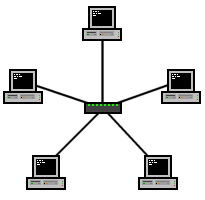
\includegraphics[scale=1]{files/img/lyaton_switch.png}
\end{center}
\end{itemize}
